% ****** Start of file apssamp.tex ******
%
%   This file is part of the APS files in the REVTeX 4.1 distribution.
%   Version 4.1r of REVTeX, August 2010
%
%   Copyright (c) 2009, 2010 The American Physical Society.
%
%   See the REVTeX 4 README file for restrictions and more information.
%
% TeX'ing this file requires that you have AMS-LaTeX 2.0 installed
% as well as the rest of the prerequisites for REVTeX 4.1
%
% See the REVTeX 4 README file
% It also requires running BibTeX. The commands are as follows:
%
%  1)  latex apssamp.tex
%  2)  bibtex apssamp
%  3)  latex apssamp.tex
%  4)  latex apssamp.tex
%
\documentclass[%
%reprint,                                   %%%%%%%%%%% this one makes it look like a paper
%superscriptaddress,
%groupedaddress,
%unsortedaddress,
%runinaddress,
%frontmatterverbose, 
preprint,                                  %%%%%%%%%%%%%%%% this one for drafting
%showpacs,preprintnumbers,
nofootinbib,
%nobibnotes,
%bibnotes,
 amsmath,amssymb,
 aps,
%pra,
%prb,
%rmp,
%prstab,
%prstper,
%floatfix,
]{revtex4-1}


%%%%%%%%%%%%%%%%%%%%%%%
\usepackage{lineno}
\linenumbers % add line numbers, draft
%%%%%%%%%%%%%%%%%%%%%%%


%%%%%%%%%%%%%%%%%%%%%%%%%%%%%%%%%%%%%%%%%%%%%%%
\usepackage{graphicx}% Include figure files                  \usepackage[draft]{graphicx}
%%%%%%%%%%%%%%%%%%%%%%%%%%%%%%%%%%%%%%%%%%%%%%%


%%%%%%%%%%%%%%%%%%%%%%%%%%%%%%%
\usepackage[printfigures]{figcaps} % send figures to end
%%%%%%%%%%%%%%%%%%%%%%%%%%%%%%%


\usepackage{dcolumn}% Align table columns on decimal point
\usepackage{bm}% bold math
%\usepackage{hyperref}% add hypertext capabilities
%\usepackage[mathlines]{lineno}% Enable numbering of text and display math
%\linenumbers\relax % Commence numbering lines

%\usepackage[showframe,%Uncomment any one of the following lines to test 
%%scale=0.7, marginratio={1:1, 2:3}, ignoreall,% default settings
%%text={7in,10in},centering,
%%margin=1.5in,
%%total={6.5in,8.75in}, top=1.2in, left=0.9in, includefoot,
%height=10in,a5paper,hmargin={3cm,0.8in},
%]{geometry}

\begin{document}

\newcommand{\wmk}{$Wm^{-1}K^{-1}$}

%\preprint{APS/123-QED}

\title{Finite size effects in simulations of thermal conductivity under lower mantle conditions}% Force line breaks with \\

\author{Ben Todd}
 \email{Corresponding  author: ee10bt@leeds.ac.uk}
\author{Stephen Stackhouse}
\author{Andrew M. Walker}
\author{Jon Mound}

\affiliation{School of Earth and Environment, University of Leeds, United Kingdom}

\date{\today}% It is always \today, today,
             %  but any date may be explicitly specified

\begin{abstract}
Knowledge of thermal conductivity is important for modelling the deep earth, but can not be measured experimentally at core mantle boundary conditions. Atomic scale simulations sidestep experimental limitations, but system size must be chosen carefully in order to determine accurate conductivity values.

Here we investigate the effects of finite simulation size and show how conductivity can be overestimated when using the direct method.
Classical molecular dynamics approaches are utilised, with the intention of constraining system parameters for future ab-initio studies.

RESULTS
\end{abstract}

\maketitle


%%%%%%%%%%%%%%%%%%%%%%%%%%%%%%%%%%
%\onecolumngrid % make one column, delete to go back to two IGNORE THIS, USE document class
%%%%%%%%%%%%%%%%%%%%%%%%%%%%%%%%%%


\section{\label{sec:intro}Introduction}

PAPERS ON PREVIOUS WORKS

PHYSICS FOCUS, EARTH SECONDARY

Thermal conductivity influences dynamic processes (such as mantle convection) and heat flow within the Earth (why important?). Until recently, lowermost mantle thermal conductivity is commonly assumed to be 10 \wmk \cite{Lay2008}, but values of 4~\textemdash~16 \wmk \cite{Goncharov2009,Lay2008,Hofmeister1999,Brown1986} (Numbers not including \citet{Manthilake2011a}) have also been proposed. 

% 

%\begin{figure}[h]
%  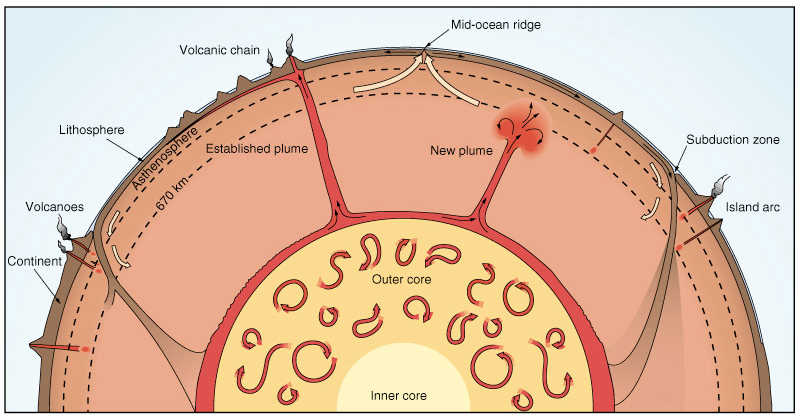
\includegraphics[width=\linewidth]{images/mantle.png}
%  \caption{Thermal conductivity of the lowermost mantle influences heat flow across the core mantle boundary (CMB),  affecting core and mantle dynamics and surface tectonic processes. Reproduced from (http://www.artinaid.com/2013/04/composition-of-the-earths-mantle/)}
%  \label{fig:mantle}
%\end{figure}

%%(Figure \ref{fig:mantle})

Experiments to determine conductivity can not be performed at the pressure/temperature conditions at the core mantle boundary (136 GPa, 4000 K). Results from low temperature experiments (\textless1500~K) are extrapolated, leading to significant uncertainty.

%\begin{figure}[h]
%  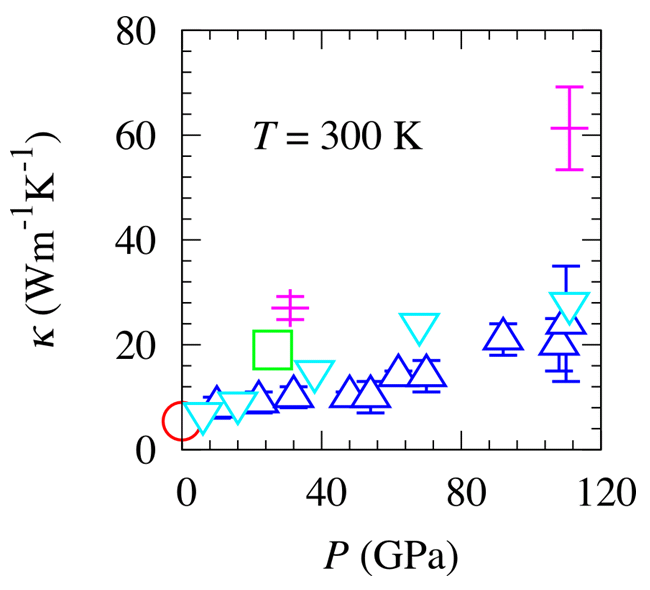
\includegraphics[width=\linewidth]{images/lattice_comparison.png}
%  \caption{Experimental results for bridgmanite at 300 K. Note the difference in conductivities for a given pressure, and the variation in gradient (pressure dependence) between studies.}
%  \label{fig:lattice_comp}
%\end{figure}

%%(Figure \ref{fig:lattice_comp})

Atomic scale calculations are not limited by the reproduction of physical conditions like experimental measurements, however they are affected by the size and shape of the simulation cell. The effects of the finite system size available for computation must be checked, systems with too few atoms are sometimes unable to reproduce the behaviour of the bulk material (REF). If the wavelength of a phonon is too long to fit into a cell, it is not able to transport heat like it should. This can happen when the system is too small  (, but also when it is too narrow. We show insufficient cross-sectional area of direct method cells influences phonon behaviour, creating a ""funneling" effect in terms of the heat transport and subsequent overestimated thermal conductivity.)


%\footnote{LAMMPS = Large-scale Atomic/Molecular Massively Parallel Simulator}

%\begin{figure}[h]
%  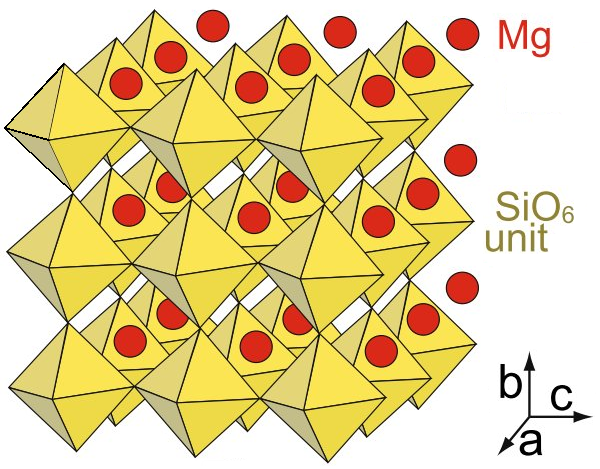
\includegraphics[width=\linewidth]{images/bridg.png}
%  \caption{Unit cell atomic structure representation of bridgmanite, the main mineral component of the lower mantle. The SiO$_6$ tetrahedra have O at the vertices and a single Si in the centre. Modified from\citet{Trønnes2009}.}
%  \label{fig:bridg}
%\end{figure}

%% Figure \ref{fig:bridg}

In section \ref{sec:methodology} we outline our computational approaches, the non-equilibrium molecular dynamics direct method and equilibrium molecular dynamics Green-Kubo method. The two methods have previously been compared (e.g. \citet{Schelling2002}), and have been found to be in good agreement. In section \ref{sec:results} we show convergence of computed conductivity with respect to simulation cell size and shape (AND PRESSURE/TEMPERATURE CONDITION?). In section \ref{sec:summary} we suggest the minimum system parameters to be utilised in similar lower mantle studies, and discuss potential future work.















\section{\label{sec:methodology}Methodology}

BASIC IDEA OF WHAT IS TO BE SHOWN

Using the classical molecular dynamics code LAMMPS\cite{Plimpton1995} (Large-scale Atomic/Molecular Massively Parallel Simulator), we calculate lattice thermal conductivities and constrain effects of finite simulation size. With the interatomic potential of \citet{Oganov2000} we simulate bridgmanite (MgSiO$_3$ perovskite), the predominant phase in the lower mantle ($\sim$75\%). 

To assess the finite-size effects within bridgmanite, we want to use larger simulation cells than those employed in previous studies. The atom counts associated with these cells (the largest cell considered having over 100,000 atoms) means an ab initio study would be impractical, necessitating the use of interatomic potentials. We expect the potentials to represent the finite size effects well, even if computed conductivities may inaccurate compared to first-principles calculations. Future work includes using density functional theory with the minimum atom count determined by this study to negate finite-size effects.  

We present the basic idea of the direct and Green-Kubo methods and show our calculations are converged with respect to simulation time, and in addition the method-specific system parameters. (REMOVE? The finite size effect analysis can be found in Section.~\ref{sec:results}, along with the comparison of both techniques' results.)




\subsection{\label{sec:method.direct}Direct method}

FLAVOURS OF DIRECT METHOD - SWAP CONSTANT HEAT OR MAINTAIN TEMPERATURE GRADIENT. SINUSOIDAL TEMPERATURE DISTRIBUTION

The direct method is the computational implementation of a typical experiment to measure thermal conductivity, using Fourier\textsc{\char13}s law to relate heat flux (q) and temperature gradient ($\nabla{T}$) to thermal conductivity (k), 
\begin{equation}
q=-k \nabla{T} \label{fourier}
\end{equation}

In the direct method energy is transferred from one group of atoms to another, creating a hot and a cold region between which heat will flow. The resultant temperature gradient is measured by calculating the temperature in individual sections of atoms along the direction of the heat flux. Simulation cells tend to be long relative to their cross-sectional area, defined as height by width (see Figure~\ref{fig:cell_dia}). All cell boundaries are periodic, meaning heat can flow out of both sides of the hot end to the cold. This results in two similar temperature gradients, which can be averaged.

\begin{figure}[h]
  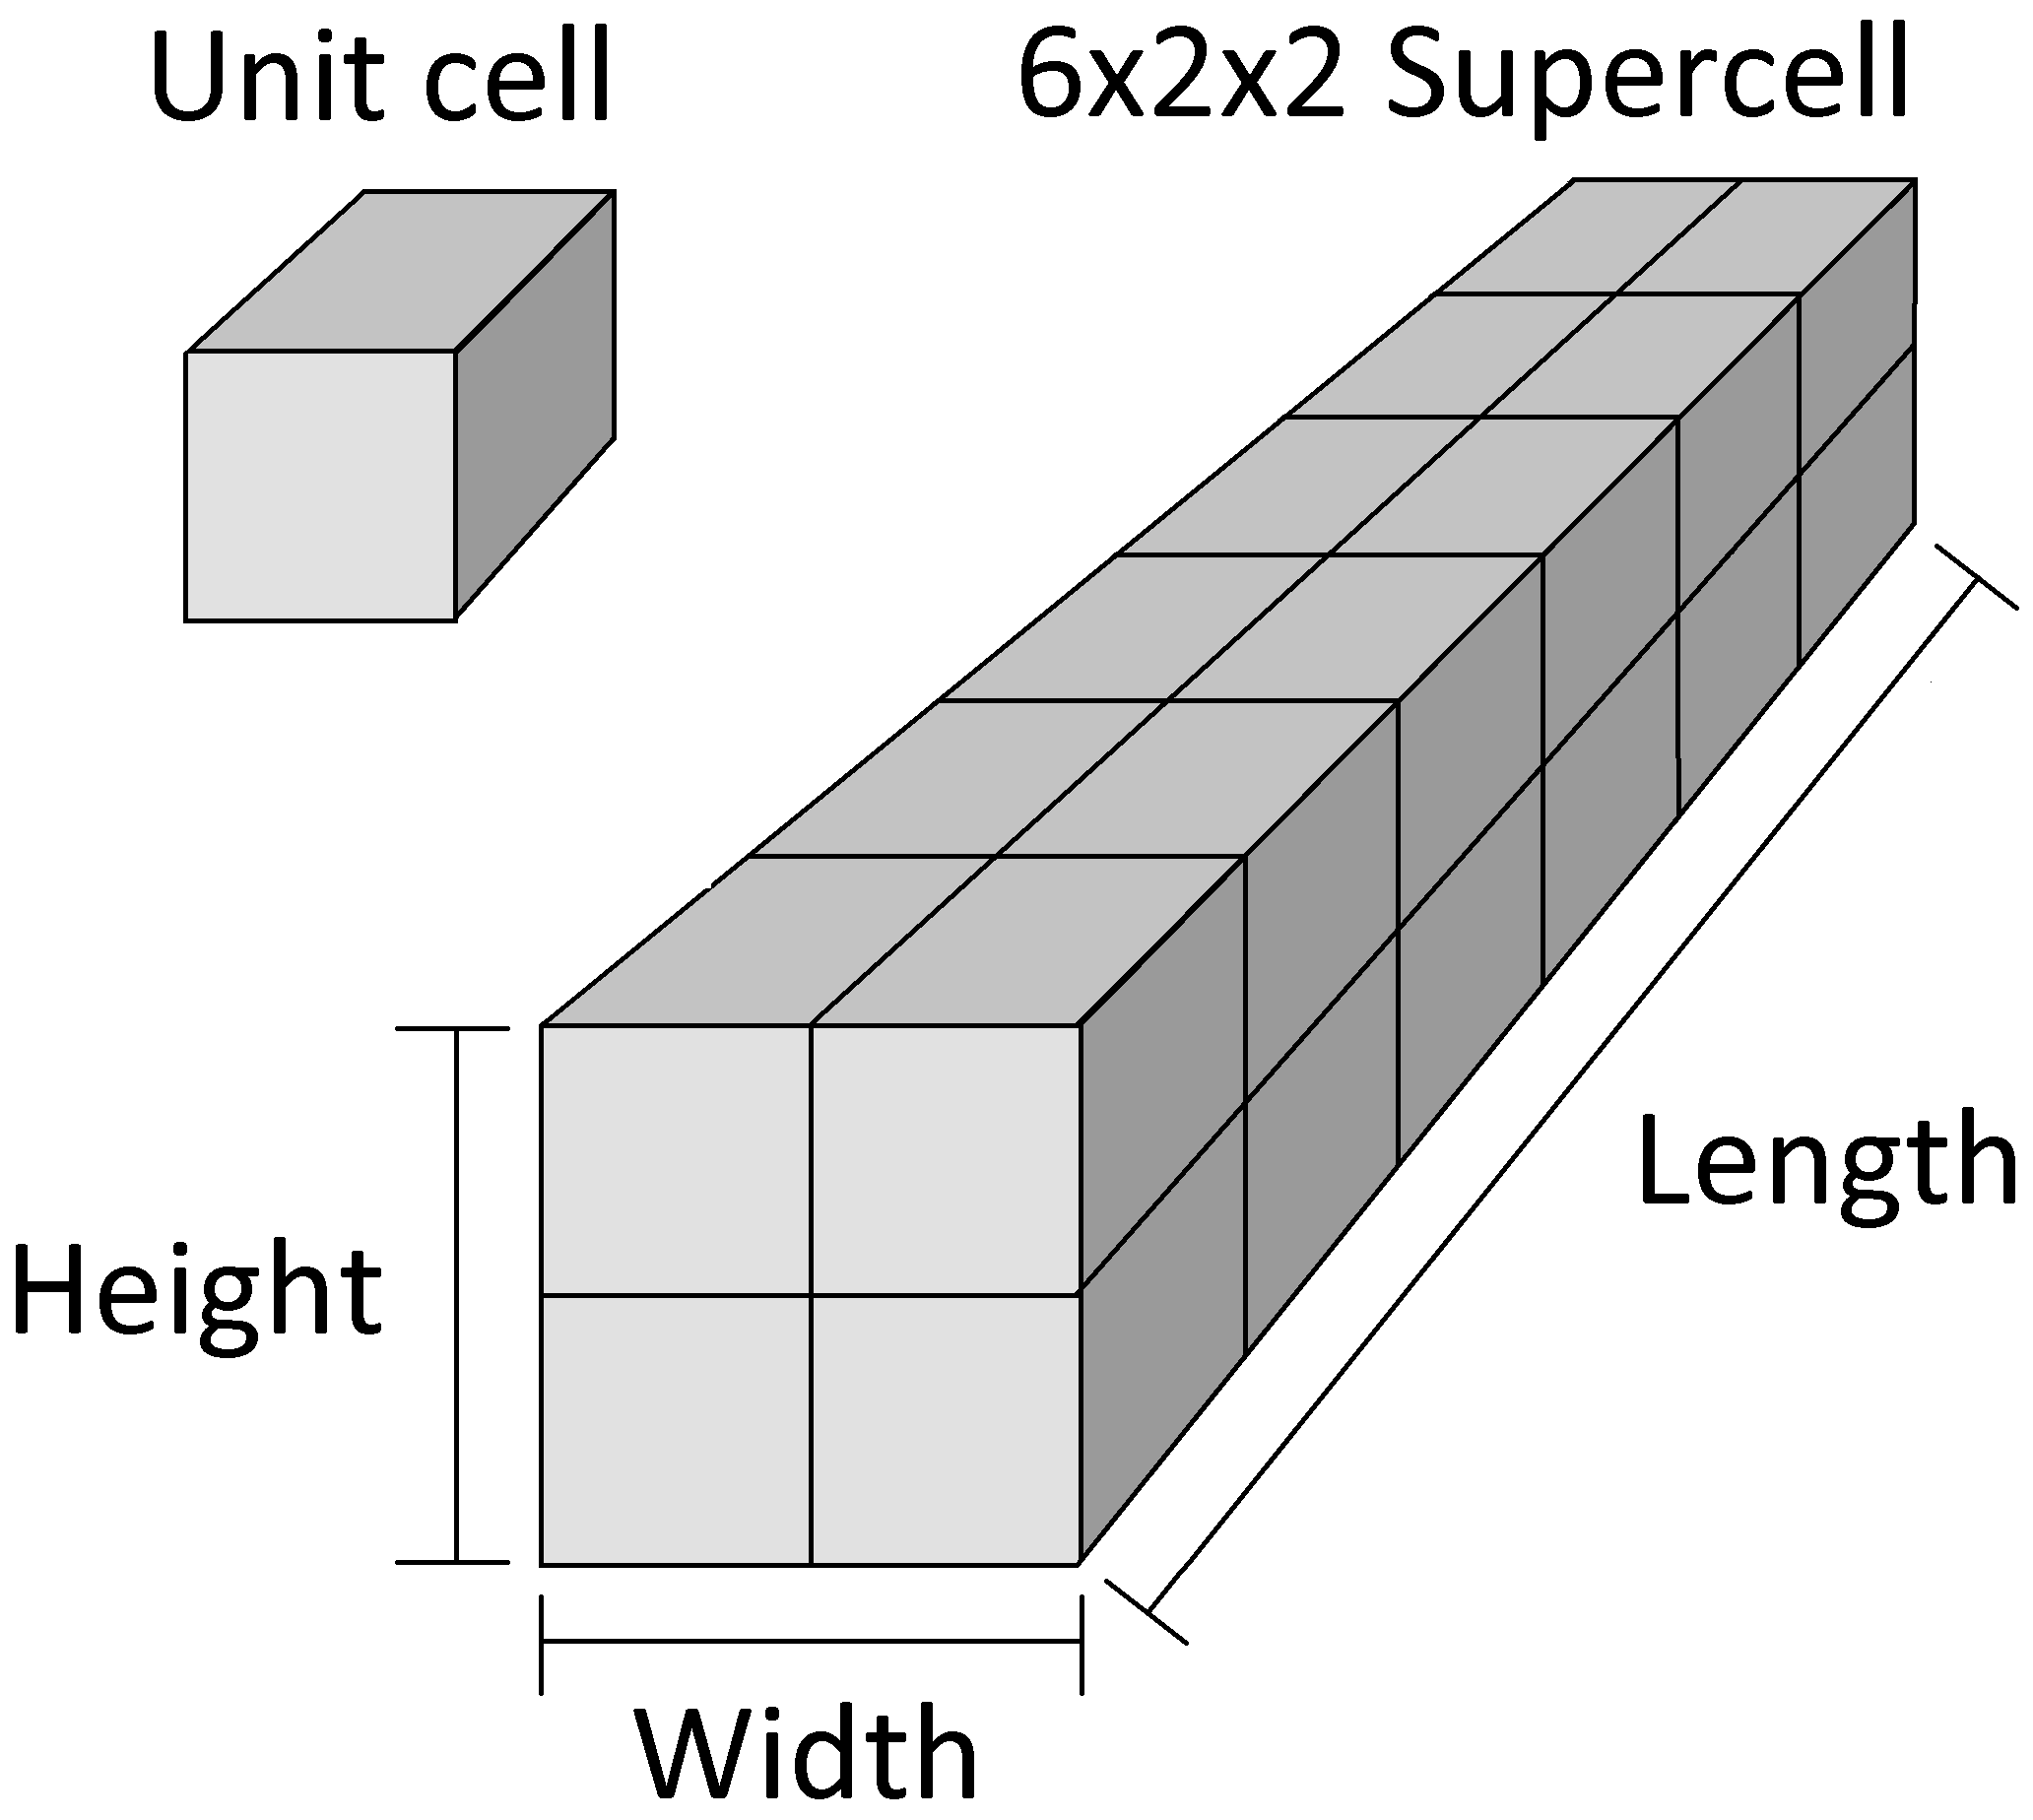
\includegraphics[width=\linewidth]{images/cell_diagram.png}
  \caption{The unit cell represents the smallest box of atoms that can be replicated to produce a crystal structure. A supercell is an arrangement of unit cells.} %Atomic structure of bridgmanite unit cell can be seen in Figure \ref{fig:bridg}.} 
\label{fig:cell_dia}
\end{figure}

%%\begin{figure}[h]
%  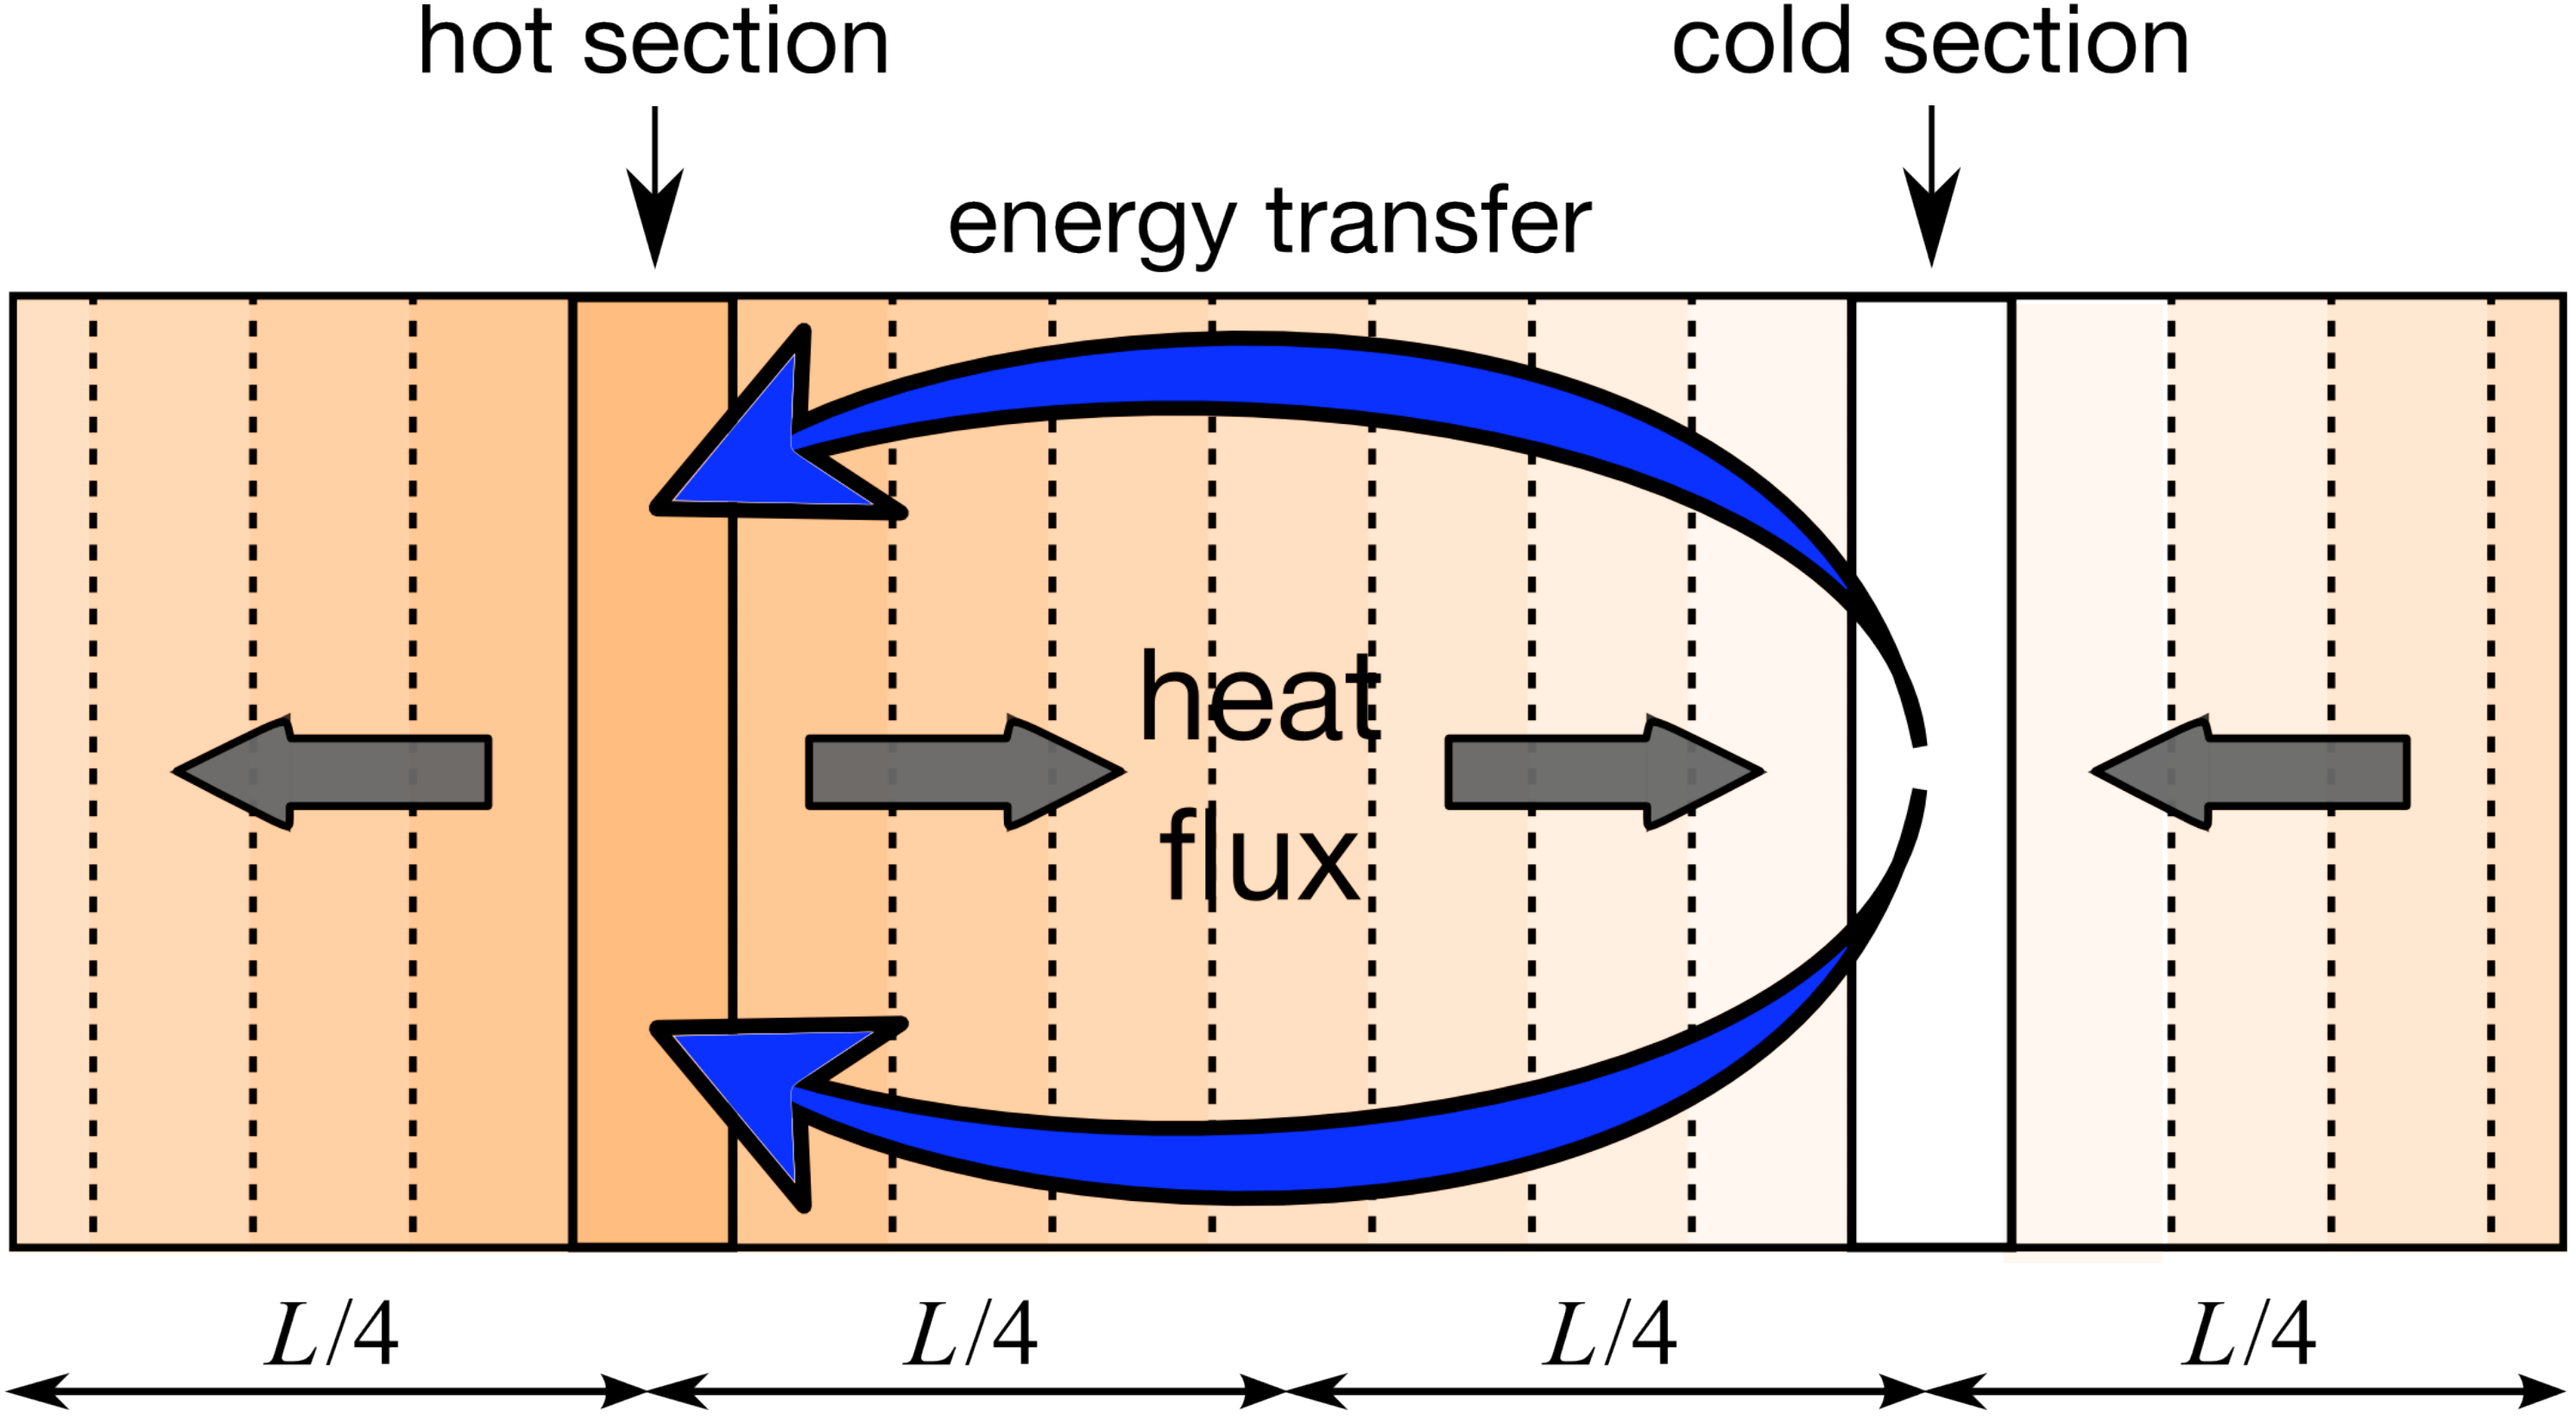
\includegraphics[width=\linewidth]{images/ss_direct_mod.png}
%  \caption{Movement and distribution of heat in the direct method. Orange to white scale represents temperature. Source: \citet{Stackhouse2015}.}
%  \label{fig:ss_direct}
%\end{figure}

%%(Figure \ref{ss_direct})

From kinetic theory, conductivities computed by the direct method ($k_L$) are dependent on length of simulation cell,
\begin{equation}
k_{L} = \frac{1}{3} C_{V} v l_{L} \label{length-dep}
\end{equation}
Where $C_v$ is the volumetric heat capacity, $v$ is the BULK SOUND VELOCITY?, and $l_L$ is the phonon mean free path. The finite size of the simulation cell truncates the mean free path, underestimating conductivity compared to that of the bulk material ($k_\infty$). Using results from simulations of varying cell length ($L$), conductivity is extrapolated to a length-independent value (where $b$ is a material dependent parameter). 

\begin{equation}
{k_{L}}^{-1} = b L^{-1} + {k_{\infty}}^{-1} \label{linear-extrap}
\end{equation}

Inverse conductivities from direct method simulations are plotted against the corresponding inverse cell lengths. A linear trend is fit to the data and extrapolated to the y-axis (at which the inverse cell length equals zero and real length equals infinity), where the intercept gives the inverse of the bulk material conductivity, see Figure \ref{fig:ideal}(REFERENCE SCHELLING HERE?).

\begin{figure}[h]
  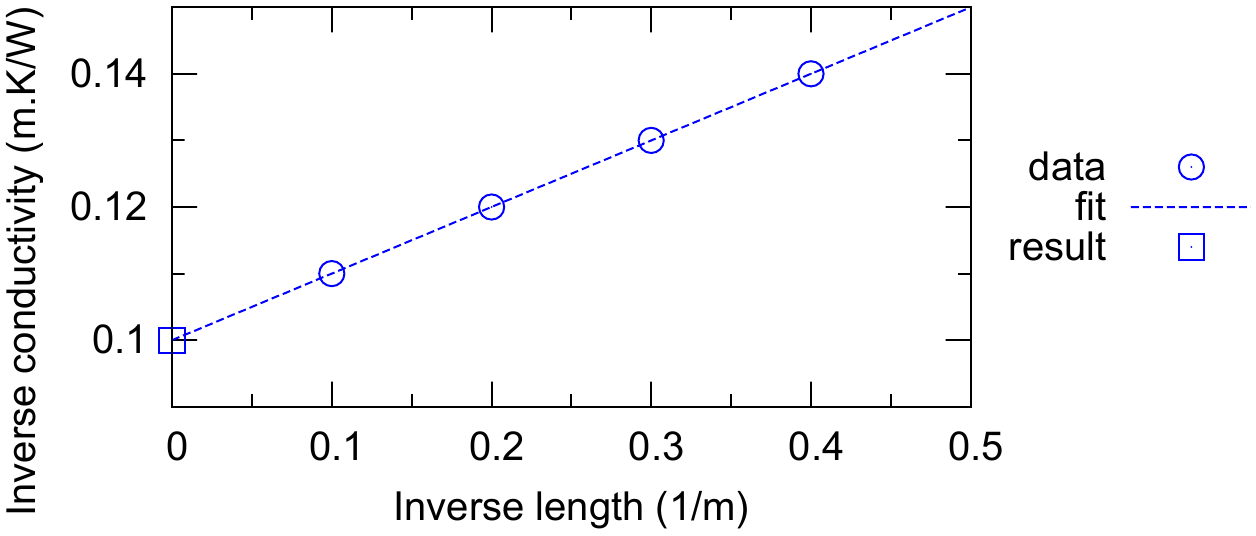
\includegraphics[width=\linewidth]{images/ideal_extrap.png}
  \caption{Idealised example of linear extrapolation procedure. Inverse computed conductivities are plotted against inverse simulation lengths. Extrapolation to y-axis gives conductivity of an infinite system length, i.e. the bulk material.}
  \label{fig:ideal}
\end{figure}

An important criterion for utilising the direct method is that the temperature gradient is sensible. Too large a range between hot and cold sections means the validity of Fourier's law is called in to question, additionally thermal conductivity is strongly temperature-dependent at upper lower-mantle conditions (1000~K). It is undesirable to have substanially different conductivities as a function of position along the length of the cell. The opposite case is also true, the difference in temperature between hot and cold sections must be larger than the uncertainty in the average system temperature. 

We typically observe fluctuations in temperature of around $\pm$50~K during temperature equilibration, and thus look for temperature ranges on the order of $\pm$100~K compared to the mean temperature. We control the magnitude of the gradient by altering the interval at which heat is exchanged. To produce the desired gradients, we find shorter intervals are required as cell length decreases, cross-sectional area increases, and system equilibrium temperature decreases. 

Figure \ref{fig:swap_int} (larger y-axis range?) shows conductivity as a function of swap interval for a 6x2x2 system at 136~GPa and 1000~K. Values are erratic for high interval / low temperature range swaps (right), and converge with decreasing swap interval (left). An interval around 10~timesteps produces suitable results for these system conditions, whilst exhibiting a sensible temperature range for the reasons mentioned above. When NVE simulations are run for a long time, there is noticable drift in the average system temperature due to the finite-distance approximation associated with molecular dynamics (???). This process is accelerated when heat is exchanged often, an important thing to check for when processing data.

\begin{figure}[h!]
  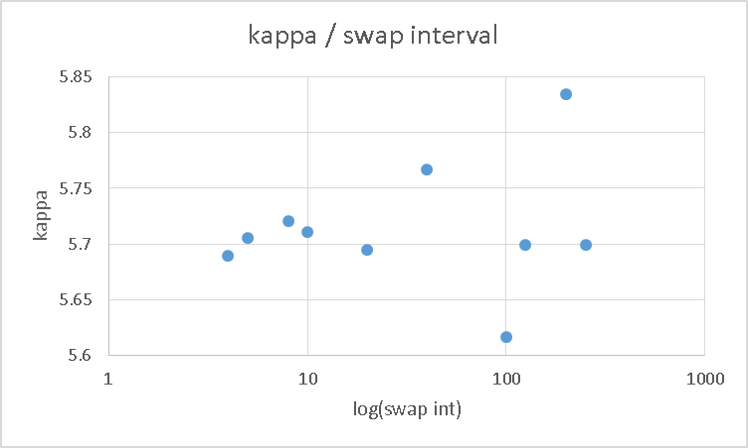
\includegraphics[width=\linewidth]{images/swap_int.png}
  \caption{CAPTION}
  \label{fig:swap_int}
\end{figure}

We ensure all calculations are run for a sufficient length of time for the conductivity value to converge (see Figure \ref{fig:kappa_conv}). When conductivity fails to converge it means either; the simulations needs to be run for longer (unlikely with our nanosecond-scale classical calculations), or the system temperature has drifted. This drift can be seen when conductivity diverges with simulation length[, and is easily checked by analysing the mean temperature of the system][too obvious / not needed?].


\begin{figure}[h!]
  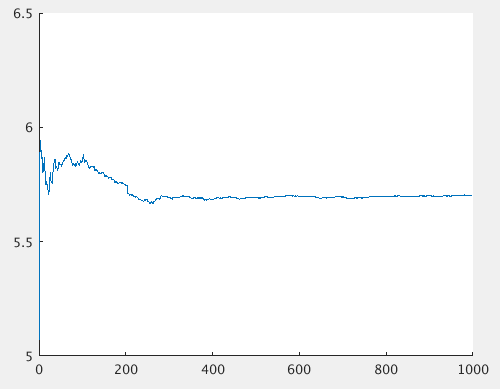
\includegraphics[width=\linewidth]{images/kappa_conv.png}
  \caption{CAPTION}
  \label{fig:kappa_conv}
\end{figure}

REFERENCE OTHER REVIEWS OF DIRECT METHOD PROCEDURE?



\subsection{\label{sec:method.gk}Green-Kubo method}

Instantaneous heat fluxes can be used to determine how energy is dissipated with in system, where brief flux events mean heat is transferred quickly indicating high thermal conductivity (and vice versa).

The Green-Kubo method uses auto-correlation functions (ACFs) to quantify time-dependence of heat fluxes (shown on Figure~\ref{fig:gk_acf}, and Equation \ref{acf-j}), in a simulation cell of roughly cubic dimensions and spatially-consistent average temperature. Auto-correlation is performed over the net heat flux series in each crystallographic direction, for a timescale up to a correlation length.

\begin{equation}
ACF_i = \left \langle J_i(0) \cdot  J_i(t) \right \rangle
\label{acf-j}
\end{equation}

\begin{figure}[h]
  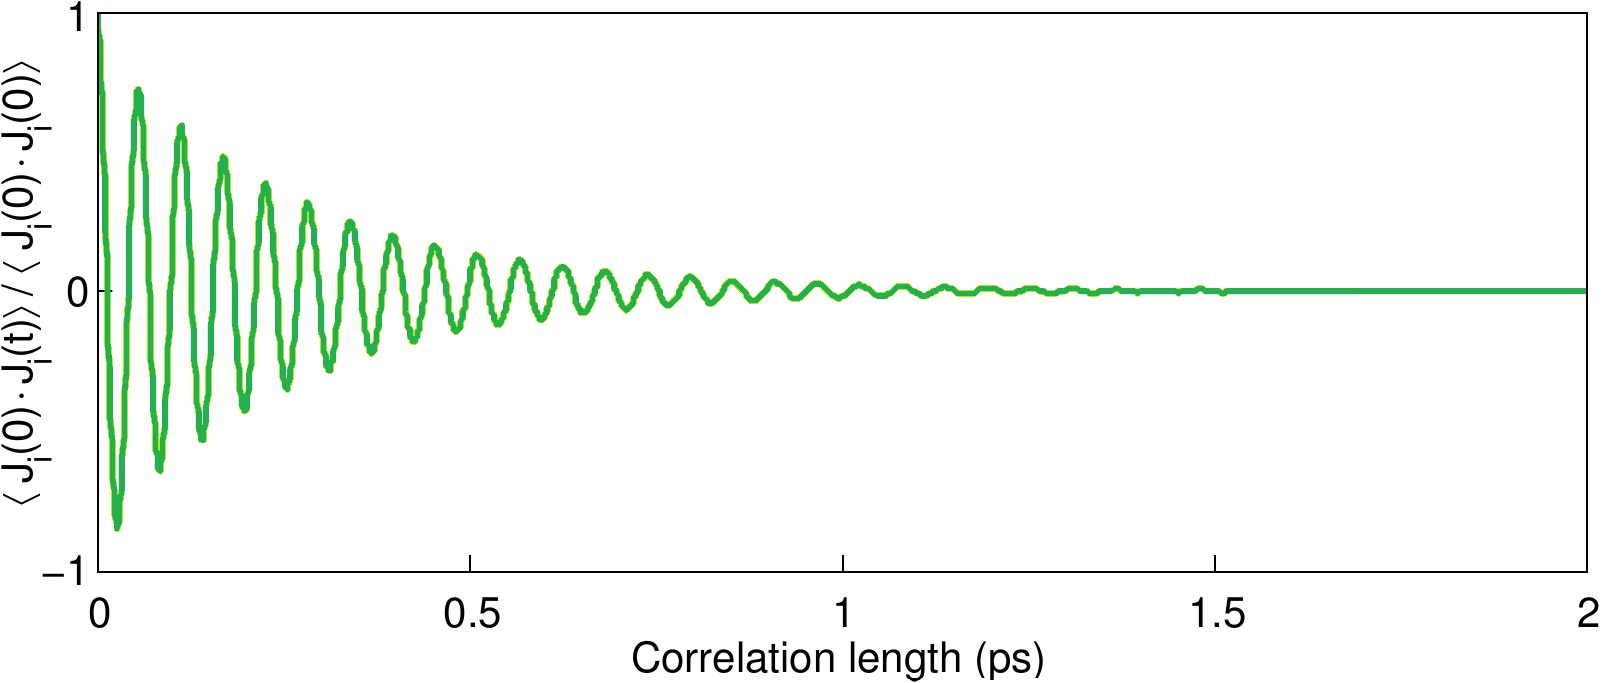
\includegraphics[width=\linewidth]{images/gk_acf.png}
  \caption{Normalised ACF. Correlation is taken over a longer length than shown on this plot (10 ps, see Figure 8 below), however the function decays to less than 1\% of its initial value at 2~ps. It continues to oscillate about zero, with a positive average value.}
  \label{fig:gk_acf}
\end{figure}

where $i$ specifies crystallographic axis, $J$ is heat flux, and $t$ is the correlation length. Integral of heat flux ACF is proportional to thermal conductivity via the Green-Kubo equation (see Figure~\ref{fig:gk_int} and Equation \ref{gk-int}), 

\begin{equation}
\kappa_i = \frac{V}{k_{B}T^2} \int_{0}^{\infty} \left \langle J_i(0) \cdot  J_i(t) \right \rangle dt ,
\label{gk-int}
\end{equation}

\begin{figure}[h]
  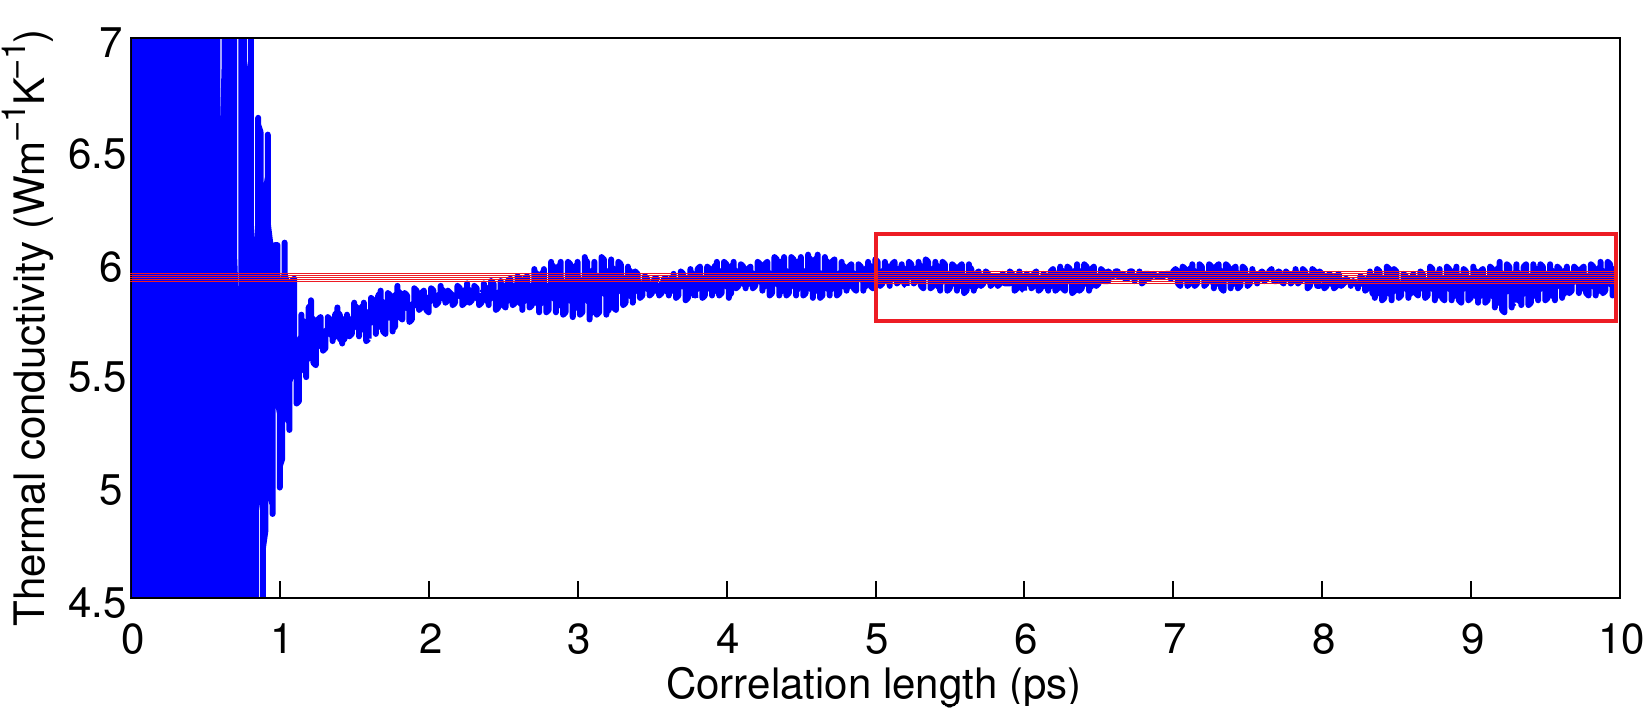
\includegraphics[width=\linewidth]{images/gk_int.png}
  \caption{Integrated ACF, multiplied by constants to get thermal conductivity. Large variation in the first 1 ps corresponds to the correlation time where the ACF is unconverged (still decaying / large oscillations). Thermal conductivity is averaged from correlation time of 5~ps - 10~ps (region in red box).}
  \label{fig:gk_int}
\end{figure}

%\begin{figure}[h!]
%  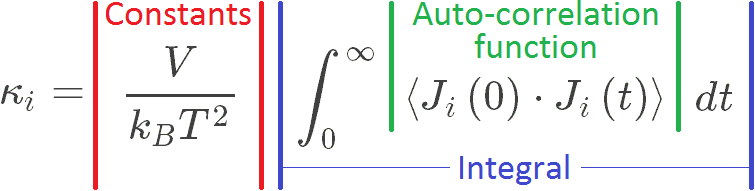
\includegraphics[width=\linewidth]{images/gk_eq.png}
%  \caption{EXPLAIN COMPONENTS}
%  \label{fig:gk_eq}
%\end{figure}

where $V$ is the simulation cell volume, $k_B$ is the Boltzmann constant, and $T$ is the average temperature of the system. In this study we use Green-Kubo results can be used as an independent check on direct method and aforementioned conductivity extrapolation, as they do not have the same finite size-effects.

Finite size-effects in Green-Kubo are much more general than those of the direct method, simply a large enough cell volume / number of atoms must be used. The bridgmanite unit cell we employ has a lattice parameter ratio (a:b:c) of roughly 1:1:1.4, meaning an approximately cubic simulation supercell should have dimensions 3x3x2, 4x4x3, 5x5x4, 6x6x4, 7x7x5 etc.



















\section{\label{sec:results}Results}

\subsection{\label{sec:results.gk}Green-Kubo method}

These parameter choices are justified by comparison with Green Kubo results (Figure~\ref{fig:gk-direct}), where the difference in computed conductivity is less than 0.4 W/m.K.

\begin{figure}[h!]
  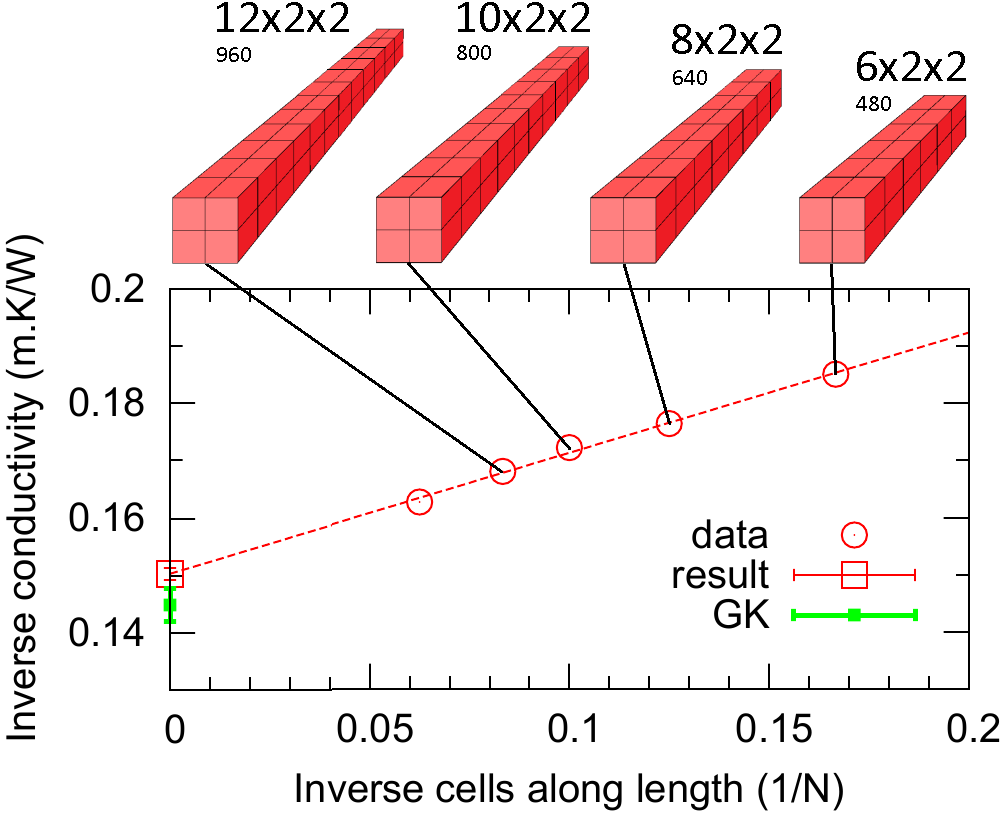
\includegraphics[width=\linewidth]{images/gk-direct.png}
  \caption{The results of Figure 9 for cross-section of 2x2 and lengths ≤ 16 unit cells. Diagrams of cell geometry are shown, with dimensions in unit cells and the number of atoms. Green-Kubo result is plotted on the y-axis for comparison with extrapolated direct method conductivity.}
  \label{fig:gk-direct}
\end{figure}



\subsection{\label{sec:results.direct}Direct method}

In addition to the expected conductivity increase with cell length, we observe two effects of finite system size.

Cells of length greater than 16 unit cells (1/N~\textless~0.0625 on Figure~\ref{fig:all_data}) show clear deviation from the expected linear trend.

\begin{figure}[h]
  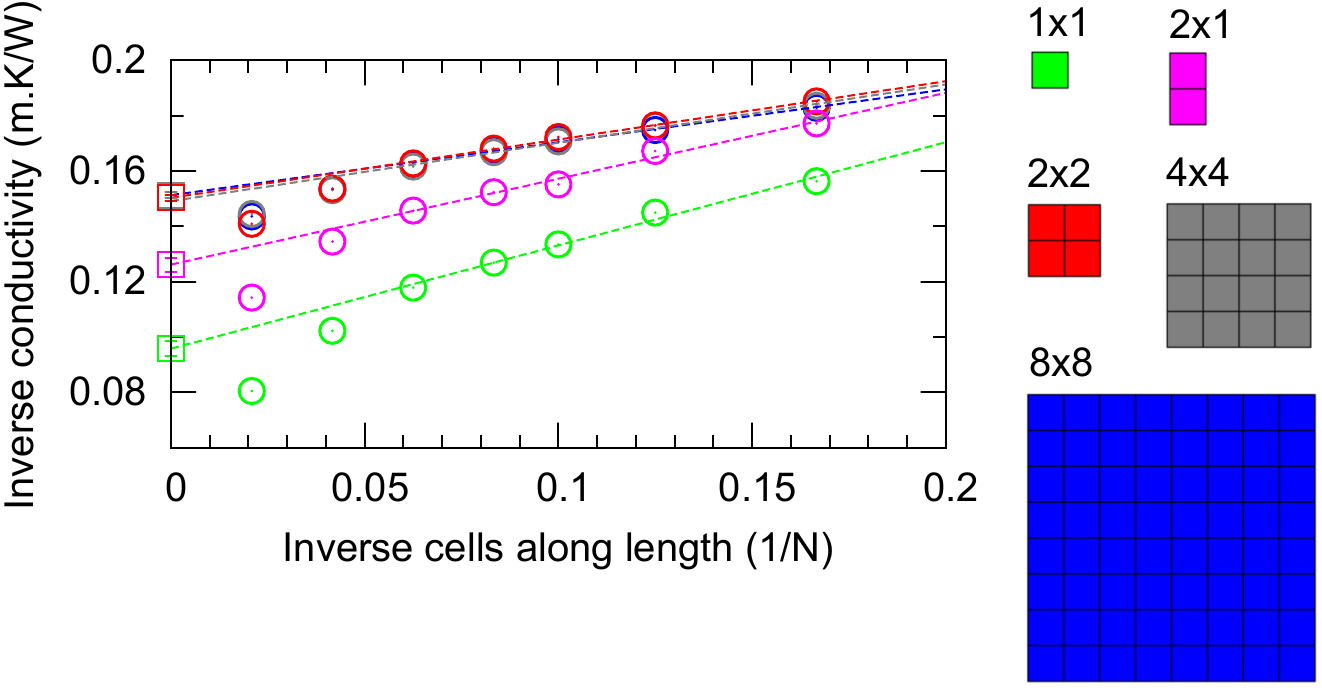
\includegraphics[width=\linewidth]{images/all_data.png}
  \caption{Compilation of direct method thermal conductivities across a range of cell shapes at 4000 K and static pressure of 136 GPa. Different cross-sections are displayed by the colour of the series, diagrams of which are shown in the legend (right). From right to left, data points correspond to lengths of 6, 8, 10, 12, 16, 24, and 48 unit cells. Inverted axes facilitate the extrapolation of conductivity to bulk material.}
  \label{fig:all_data}
\end{figure}

As it is inappropriate to fit non-linear data, we ignore conductivity results from the long cells and perform the extrapolation only where a linear trend is suitable.

While the extrapolation procedure requires multiple cell lengths, the effects of cell cross-sectional area are not considered. 

We show cells with small cross-section overestimate conductivity, the magnitude of which decreases with increasing area. 

A sufficient cross-sectional area for bridgmanite is greater than 2x2, as extrapolated conductivities converge. 

To obtain thermal conductivity results that are converged with respect to direct method system size, we use the following criteria,

Cell lengths $\leq$ 16 unit cells

Cross-section = 2x2 unit cells





















\section{\label{sec:summary}Summary and conclusion}

For bridgmanite, we show that use of the direct method for calculation of thermal conductivity will lead to an overestimate if the simulation cell is too long (\textgreater 16 unit cells).

Small cross-sectional areas (\textless 2x2 unit cells) also overestimate the thermal conductivity.

This informs future work using Density Functional Theory, and will allow a model of lower mantle conductivity considering composition to be established.

Sellan et al. state the non-linearity observed when performing the extrapolation procedure is actually the true conductivity-length dependence, and any linear regime is undersampling a portion of the relationship (WHAT CAUSES DEVIATION FROM LINEAR EQUATION???). System sizes smaller than the dominant phonon mean free path wavelength incorrectly produce a linear relationship, and underestimate thermal conductivity. HOPEFULLY RELATION WITH MY GREEN-KUBO PROVES SENSIBLE EXTRAPOLATION. HOPEFULLY MY CELL LENGTHS LONGER THAN DOMINANT PHONON MFP IF CALCULATED.

(ASSUMING THE RESULTS ARE CORRECT) We see the non-linear region as described by Sellan et al. for the cell length of 6 unit cells at 1000~K, which has individually higher conductivity than expected from the linear fit through data points corresponding to lengths of 8-16 unit cells. When included in the extrapolation, this reduces the gradient of the fit, raising the intercept and thus causing conductivity to be underestimated.

At temperature of 4000~K, the 6 length cell is inline with the fit through cells with length less than 16 unit cells. As the ratio of cell length to phonon MFP increases with temperature, we believe the onset of divergence as described by Sellan et al. moves to the right (???). A shorter MFP needs a shorter cell length to display divergent conductivity, of which we have not sampled. DOING THE DIRECT METHOD WITH CELLS OF LENGTH LESS THAN 6 UNIT CELLS AT ANY TEMPERATURE IS A BAD IDEA BECAUSE ... 

(ASSUMING 8 LENGTH IS LONGER THE MFP AND NOT 24) Sellan et al. do not observe the extreme non-linearity for cells longer than 24 unit cells length, which causes great overestimation of conductivity (ASSUMING GK IS CORRECT). Hu et al. however do observe this effect, the estimation of conductivity with increasing length for a constant CSA. Once the aspect ratio of the system (length:CSA) exceeds a critical value, a 3D system begins to exhibit behaviour seen in 1D systems. Whereas true 1D systems show length-divergent conductivity because of ballistic phonon transport, Hu et al. state 3D systems with periodic boundary conditions behaving in a 1D fashion is due to sparse phonon phase sampling. We find conductivity is definitely dependent on CSA, but we were not able to increase CSA enough to eliminate aspect ratio-dependent divergence. This does support our conclusion ignoring long cell lengths however, in order to keep the aspect ratio in a reasonable limit. (EVEN THOUGH 48x8x8 HAS A SMALLER RATIO than 8x2x2?)

\begin{acknowledgements}
Thank you NERC

"We also acknowledge the use of high performance computing provided by Advanced Research Computing at the University of Leeds."

ANDREW HAS SOMETHING TO ADD (AMW IRF from NERC w/ grant code)
\end{acknowledgements}

\bibliography{paper1}



\end{document}


